\documentclass{standalone}
\usepackage{tikz}
\usetikzlibrary{patterns, positioning}


\begin{document}
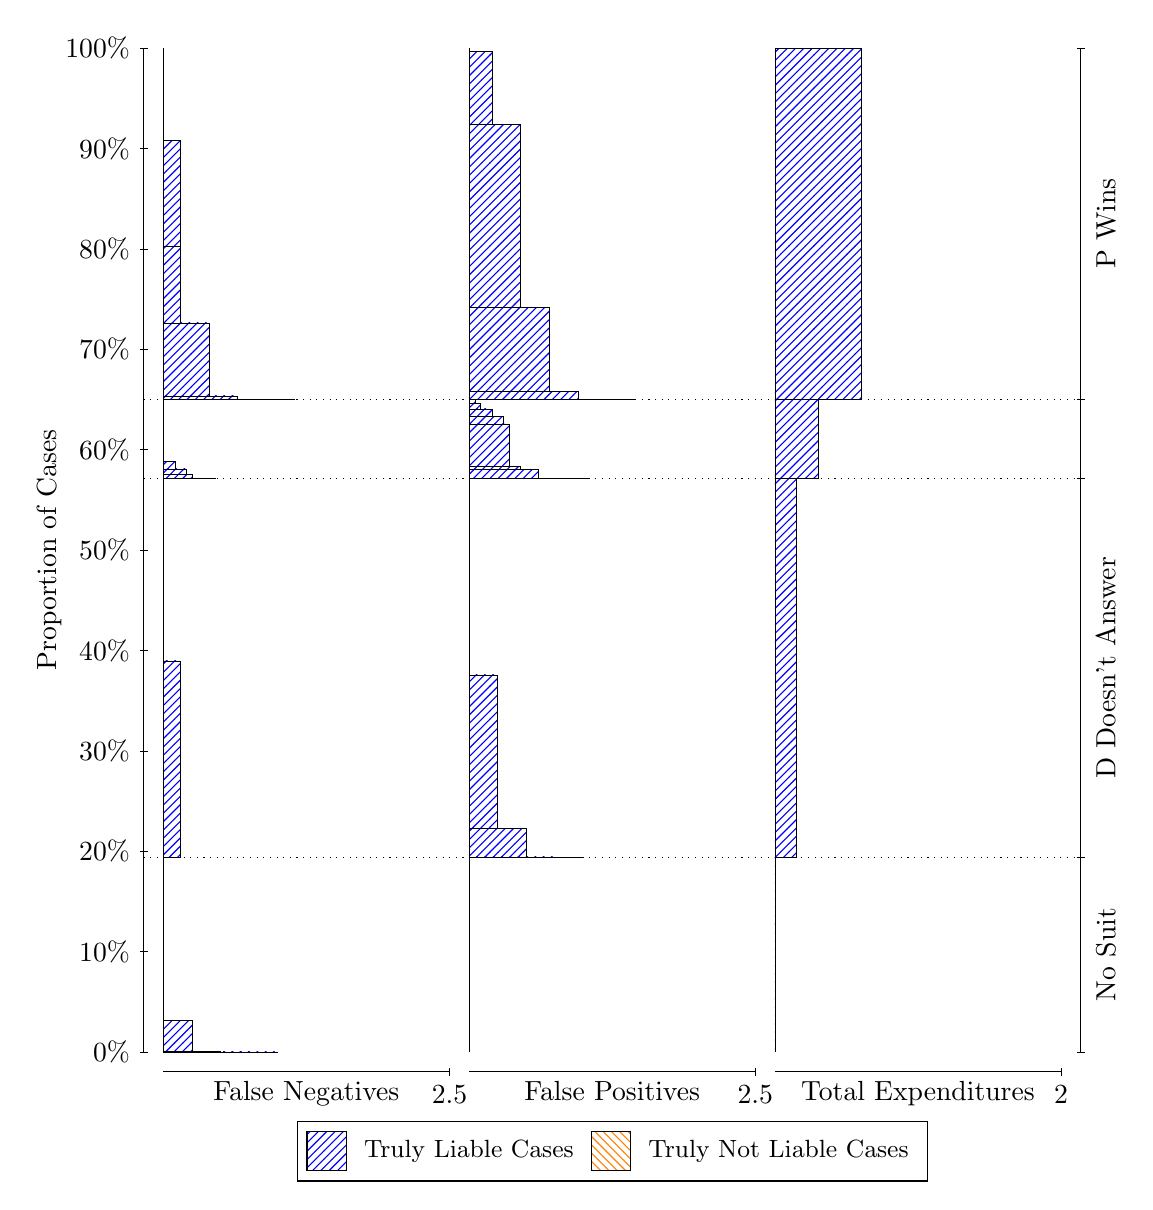
\begin{tikzpicture}
\draw[black, very thin] (1.5,1.75) -- (1.5,14.5);
\node[rotate=90, text=black, anchor=center] at (0.3, 8.125) {Proportion of Cases};
\draw[black, very thin] (1.45,1.75) -- (1.55,1.75);
\node[text=black, anchor=east] at (1.45, 1.75) {0\%};
\draw[black, very thin] (1.45,3.025) -- (1.55,3.025);
\node[text=black, anchor=east] at (1.45, 3.025) {10\%};
\draw[black, very thin] (1.45,4.3) -- (1.55,4.3);
\node[text=black, anchor=east] at (1.45, 4.3) {20\%};
\draw[black, very thin] (1.45,5.575) -- (1.55,5.575);
\node[text=black, anchor=east] at (1.45, 5.575) {30\%};
\draw[black, very thin] (1.45,6.85) -- (1.55,6.85);
\node[text=black, anchor=east] at (1.45, 6.85) {40\%};
\draw[black, very thin] (1.45,8.125) -- (1.55,8.125);
\node[text=black, anchor=east] at (1.45, 8.125) {50\%};
\draw[black, very thin] (1.45,9.4) -- (1.55,9.4);
\node[text=black, anchor=east] at (1.45, 9.4) {60\%};
\draw[black, very thin] (1.45,10.675) -- (1.55,10.675);
\node[text=black, anchor=east] at (1.45, 10.675) {70\%};
\draw[black, very thin] (1.45,11.95) -- (1.55,11.95);
\node[text=black, anchor=east] at (1.45, 11.95) {80\%};
\draw[black, very thin] (1.45,13.225) -- (1.55,13.225);
\node[text=black, anchor=east] at (1.45, 13.225) {90\%};
\draw[black, very thin] (1.45,14.5) -- (1.55,14.5);
\node[text=black, anchor=east] at (1.45, 14.5) {100\%};

\draw[black, very thin] (13.4,1.75) -- (13.4,14.5);
\draw[black, very thin] (13.35,1.75) -- (13.45,1.75);
\node[anchor=west] at (13.35, 1.75) {};
\draw[black, very thin] (13.35,4.2243) -- (13.45,4.2243);
\node[anchor=west] at (13.35, 4.2243) {};
\draw[black, very thin] (13.35,9.0334) -- (13.45,9.0334);
\node[anchor=west] at (13.35, 9.0334) {};
\draw[black, very thin] (13.35,10.038) -- (13.45,10.038);
\node[anchor=west] at (13.35, 10.038) {};
\draw[black, very thin] (13.35,14.5) -- (13.45,14.5);
\node[anchor=west] at (13.35, 14.5) {};

\draw[black, very thin, pattern color=blue, pattern=north east lines] (1.75,1.75) rectangle (3.2033,1.75);
\draw[black, very thin, pattern color=blue, pattern=north east lines] (1.75,1.75) rectangle (2.84,1.75);
\draw[black, very thin, pattern color=blue, pattern=north east lines] (1.75,1.75) rectangle (2.4767,1.7535);
\draw[black, very thin, pattern color=blue, pattern=north east lines] (1.75,1.7535) rectangle (2.1133,2.1551);
\draw[black, very thin, pattern color=orange, pattern=north west lines] (1.75,2.1551) rectangle (1.75,2.1551);
\draw[black, very thin, pattern color=blue, pattern=north east lines] (1.75,2.1551) rectangle (1.75,4.2243);
\draw[black, very thin, pattern color=blue, pattern=north east lines] (1.75,4.2243) rectangle (1.968,6.7177);
\draw[black, very thin, pattern color=orange, pattern=north west lines] (1.75,6.7177) rectangle (1.75,6.7177);
\draw[black, very thin, pattern color=blue, pattern=north east lines] (1.75,6.7177) rectangle (1.75,9.0334);
\draw[black, very thin, pattern color=blue, pattern=north east lines] (1.75,9.0334) rectangle (2.404,9.0335);
\draw[black, very thin, pattern color=blue, pattern=north east lines] (1.75,9.0335) rectangle (2.2587,9.0386);
\draw[black, very thin, pattern color=blue, pattern=north east lines] (1.75,9.0386) rectangle (2.1133,9.0859);
\draw[black, very thin, pattern color=blue, pattern=north east lines] (1.75,9.0859) rectangle (2.0407,9.1545);
\draw[black, very thin, pattern color=blue, pattern=north east lines] (1.75,9.1545) rectangle (1.8953,9.2527);
\draw[black, very thin, pattern color=orange, pattern=north west lines] (1.75,9.2527) rectangle (1.75,9.2527);
\draw[black, very thin, pattern color=blue, pattern=north east lines] (1.75,9.2527) rectangle (1.75,10.038);
\draw[black, very thin, pattern color=blue, pattern=north east lines] (1.75,10.038) rectangle (3.4213,10.038);
\draw[black, very thin, pattern color=blue, pattern=north east lines] (1.75,10.038) rectangle (3.058,10.038);
\draw[black, very thin, pattern color=blue, pattern=north east lines] (1.75,10.038) rectangle (2.6947,10.082);
\draw[black, very thin, pattern color=blue, pattern=north east lines] (1.75,10.082) rectangle (2.3313,11.01);
\draw[black, very thin, pattern color=blue, pattern=north east lines] (1.75,11.01) rectangle (1.968,11.98);
\draw[black, very thin, pattern color=blue, pattern=north east lines] (1.75,11.98) rectangle (1.968,13.328);
\draw[black, very thin, pattern color=orange, pattern=north west lines] (1.75,13.328) rectangle (1.75,13.328);
\draw[black, very thin, pattern color=blue, pattern=north east lines] (1.75,13.328) rectangle (1.75,14.5);
\draw[black, very thin, pattern color=orange, pattern=north west lines] (5.6333,1.75) rectangle (5.6333,1.75);
\draw[black, very thin, pattern color=blue, pattern=north east lines] (5.6333,1.75) rectangle (5.6333,4.2243);
\draw[black, very thin, pattern color=orange, pattern=north west lines] (5.6333,4.2243) rectangle (7.0867,4.2243);
\draw[black, very thin, pattern color=blue, pattern=north east lines] (5.6333,4.2243) rectangle (7.0867,4.2243);
\draw[black, very thin, pattern color=blue, pattern=north east lines] (5.6333,4.2243) rectangle (6.7233,4.2269);
\draw[black, very thin, pattern color=blue, pattern=north east lines] (5.6333,4.2269) rectangle (6.36,4.5868);
\draw[black, very thin, pattern color=blue, pattern=north east lines] (5.6333,4.5868) rectangle (5.9967,6.54);
\draw[black, very thin, pattern color=blue, pattern=north east lines] (5.6333,6.54) rectangle (5.6333,9.0334);
\draw[black, very thin, pattern color=orange, pattern=north west lines] (5.6333,9.0334) rectangle (7.1593,9.0334);
\draw[black, very thin, pattern color=blue, pattern=north east lines] (5.6333,9.0334) rectangle (7.1593,9.0334);
\draw[black, very thin, pattern color=orange, pattern=north west lines] (5.6333,9.0334) rectangle (7.014,9.0334);
\draw[black, very thin, pattern color=blue, pattern=north east lines] (5.6333,9.0334) rectangle (7.014,9.0334);
\draw[black, very thin, pattern color=orange, pattern=north west lines] (5.6333,9.0334) rectangle (6.8687,9.0334);
\draw[black, very thin, pattern color=blue, pattern=north east lines] (5.6333,9.0334) rectangle (6.8687,9.0336);
\draw[black, very thin, pattern color=blue, pattern=north east lines] (5.6333,9.0336) rectangle (6.796,9.0336);
\draw[black, very thin, pattern color=blue, pattern=north east lines] (5.6333,9.0336) rectangle (6.6507,9.0339);
\draw[black, very thin, pattern color=blue, pattern=north east lines] (5.6333,9.0339) rectangle (6.5053,9.1467);
\draw[black, very thin, pattern color=blue, pattern=north east lines] (5.6333,9.1467) rectangle (6.4327,9.1501);
\draw[black, very thin, pattern color=blue, pattern=north east lines] (5.6333,9.1501) rectangle (6.2873,9.1907);
\draw[black, very thin, pattern color=blue, pattern=north east lines] (5.6333,9.1907) rectangle (6.142,9.7253);
\draw[black, very thin, pattern color=blue, pattern=north east lines] (5.6333,9.7253) rectangle (6.0693,9.8189);
\draw[black, very thin, pattern color=blue, pattern=north east lines] (5.6333,9.8189) rectangle (5.924,9.9171);
\draw[black, very thin, pattern color=blue, pattern=north east lines] (5.6333,9.9171) rectangle (5.7787,9.9856);
\draw[black, very thin, pattern color=blue, pattern=north east lines] (5.6333,9.9856) rectangle (5.706,10.033);
\draw[black, very thin, pattern color=blue, pattern=north east lines] (5.6333,10.033) rectangle (5.6333,10.038);
\draw[black, very thin, pattern color=orange, pattern=north west lines] (5.6333,10.038) rectangle (7.7407,10.038);
\draw[black, very thin, pattern color=blue, pattern=north east lines] (5.6333,10.038) rectangle (7.7407,10.038);
\draw[black, very thin, pattern color=orange, pattern=north west lines] (5.6333,10.038) rectangle (7.3773,10.038);
\draw[black, very thin, pattern color=blue, pattern=north east lines] (5.6333,10.038) rectangle (7.3773,10.039);
\draw[black, very thin, pattern color=orange, pattern=north west lines] (5.6333,10.039) rectangle (7.014,10.039);
\draw[black, very thin, pattern color=blue, pattern=north east lines] (5.6333,10.039) rectangle (7.014,10.136);
\draw[black, very thin, pattern color=orange, pattern=north west lines] (5.6333,10.136) rectangle (6.6507,10.136);
\draw[black, very thin, pattern color=blue, pattern=north east lines] (5.6333,10.136) rectangle (6.6507,11.21);
\draw[black, very thin, pattern color=orange, pattern=north west lines] (5.6333,11.21) rectangle (6.2873,11.21);
\draw[black, very thin, pattern color=blue, pattern=north east lines] (5.6333,11.21) rectangle (6.2873,13.528);
\draw[black, very thin, pattern color=blue, pattern=north east lines] (5.6333,13.528) rectangle (5.924,14.456);
\draw[black, very thin, pattern color=blue, pattern=north east lines] (5.6333,14.456) rectangle (5.6333,14.5);
\draw[black, very thin, pattern color=orange, pattern=north west lines] (9.5167,1.75) rectangle (9.5167,1.75);
\draw[black, very thin, pattern color=blue, pattern=north east lines] (9.5167,1.75) rectangle (9.5167,4.2243);
\draw[black, very thin, pattern color=orange, pattern=north west lines] (9.5167,4.2243) rectangle (9.7892,4.2243);
\draw[black, very thin, pattern color=blue, pattern=north east lines] (9.5167,4.2243) rectangle (9.7892,9.0334);
\draw[black, very thin, pattern color=orange, pattern=north west lines] (9.5167,9.0334) rectangle (10.062,9.0334);
\draw[black, very thin, pattern color=blue, pattern=north east lines] (9.5167,9.0334) rectangle (10.062,10.038);
\draw[black, very thin, pattern color=orange, pattern=north west lines] (9.5167,10.038) rectangle (10.607,10.038);
\draw[black, very thin, pattern color=blue, pattern=north east lines] (9.5167,10.038) rectangle (10.607,14.5);
\draw[black, dotted] (1.5,4.2243) -- (13.4,4.2243);
\draw[black, dotted] (1.5,9.0334) -- (13.4,9.0334);
\draw[black, dotted] (1.5,10.038) -- (13.4,10.038);
\draw[black, very thin] (1.75,1.5) -- (5.3833,1.5);
\node[text=black, anchor=north] at (3.5667, 1.5) {False Negatives};
\draw[black, very thin] (5.3833,1.45) -- (5.3833,1.55);
\node[text=black, anchor=north] at (5.3833, 1.45) {2.5};

\draw[black, very thin] (5.6333,1.5) -- (9.2667,1.5);
\node[text=black, anchor=north] at (7.45, 1.5) {False Positives};
\draw[black, very thin] (9.2667,1.45) -- (9.2667,1.55);
\node[text=black, anchor=north] at (9.2667, 1.45) {2.5};

\draw[black, very thin] (9.5167,1.5) -- (13.15,1.5);
\node[text=black, anchor=north] at (11.333, 1.5) {Total Expenditures};
\draw[black, very thin] (13.15,1.45) -- (13.15,1.55);
\node[text=black, anchor=north] at (13.15, 1.45) {2};

\node[text=black, centered, rotate=90] at (13.72, 2.9871) {No Suit};
\node[text=black, centered, rotate=90] at (13.72, 6.6288) {D Doesn't Answer};

\node[text=black, centered, rotate=90] at (13.72, 12.269) {P Wins};

\draw (7.449999999999999,1.5) node[draw=none] (baseCoordinate) {};
\begin{scope}[align=center]
        \matrix[scale=0.5, draw=black, below=0.5cm of baseCoordinate, nodes={draw}, column sep=0.1cm]{
            \node[rectangle, draw, minimum width=0.5cm, minimum height=0.5cm, pattern color=blue, pattern=north east lines] {}; &
            \node[draw=none, font=\small, text=black] (B) {Truly Liable Cases}; &
            \node[rectangle, draw, minimum width=0.5cm, minimum height=0.5cm, pattern color=orange, pattern=north west lines] {}; &
            \node[draw=none, font=\small, text=black] (B) {Truly Not Liable Cases}; \\
            };
\end{scope}

\end{tikzpicture}
\end{document}